\chapter{Further Work}
\label{chap:Further}

The main task of this project was to create a prototype illustrating a way to facilitate digital city spaces as well as encouraging increased use of existing city spaces. However the full scope of creating such a service with all the sufficient functionalities and incentives for people to use is not a feasible task for a group with our level of resources in the short timeframe provided. Therefore this chapter will detail different features and functionalities that we believe should, or in some cases must, be completed before the product can achieve a successful launch. The first section will detail the work that is required before an eventual launch. This section covers legal issues and functionalities that were not prioritized during the project work. The section after it describes and expands upon features we believe should be implemented or considered in the future, but which can be added after launch.

\section{Required for Launch}
\label{sec:FurtherRequired}

\subsection{Lacking Functionalities}
\label{subsec:FurtherRequiredLacking}

At the point of completion there were some functionalities that originally were intended to be included in the delivered product but due to time constraints were not considered of high enough priority to complete with the existing time constraints. Additionally there were some known bugs and faults that were not fixed in time for delivery. Most of these should be completed if an attempt at a product launch is made. The list of these will be gone through in detail below.

\begin{figure}[ht!]
  \centering
  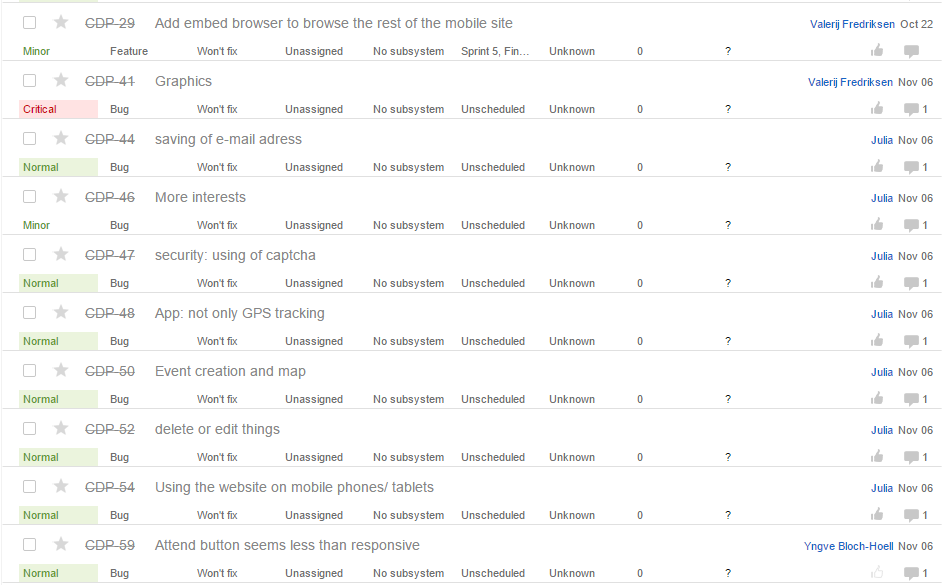
\includegraphics[width=\linewidth]{./FurtherWork/img/missingfunc}
  \caption{List of missing functionalities and known bugs at time of delivery}
  \label{fig:FurtherRequredLackingMissingFunc}
\end{figure}

\begin{description}
  \item[Add embedded browser to browse the rest of the site] \hfill \\ This refers to the mobile app and developing the app as an embedded browser, which is an easy way to reuse the existing web application. This solution will use the underlying features of the web application, but the browser in the app must handle displaying the site in a user friendly fashion for a mobile application. This would include resizing of some elements and possibly a solution for displaying the map only when required in order to effectively utilize screen space on small devices.
  \item[Graphics] \hfill \\ This point concerns the creation of several versions of the logo to be displayed in different circumstances. This includes icons for the site, icon for displaying in browser tabs, and a feature graphic for use on Google Play.
  \item[Saving of email address] \hfill \\ This point is about the linking of a user account to an email account. This will make providing user services easier and will provide a means of user verification. A field for email address should be included in the user registration form, and the activation of a user account might require a verification link sent to the registered email address.
  \item[More interests] \hfill \\ At the time of delivery the system only includes a few interests used for illustration purposes. Before the product is launched it is important to add more interests to the system to cover more activities. However it may not be feasible to add all relevant interests to the system before launch as a complete charting would be almost impossible to conduct, and different areas may have location specific interests. As time goes by completely new activities may arise as well and adding these before they exist is impossible. Solutions to this is discussed later in this chapter.
  \item[Security: Using CAPTCHA] \hfill \\ Implementing a CAPTCHA solution for customer registration and possibly for other features as well will hinder the use of an automated script to perform these actions. A CAPTCHA is a test most often requiring a user to correctly identify a set of letters and numbers from a picture.
  \item[App: not only GPS tracking] \hfill \\ This point refers to the mobile application currently using the location saved in the image file when uploading a picture. The result of this is that a picture will use the location it was taken on if that information exists in the file. If a user attempts to upload a picture without a location the users will not be able to do so as the picture will be rejected by the system. Solving this could be done using a map solution where the user can pinpoint the location of the picture, this solution should also include a feature for searching in the map for places and addresses.
  \item[Delete or edit things] \hfill \\ In its current state the system does not allow users to edit or delete comments, user profiles, events, or photos. In the future system functions allowing a user to edit and delete content created by that user should be implemented, and users should have the option to delete their profile as well if they no longer wish to use the service.
  \item[Using the website on mobile phones/tablets] \hfill \\ Accessing the website with a browser for a mobile device does not function properly. In the future development of this project solving this should be considered. This feature becomes less important if mobile applications are created.
  \item[Attend button seems less than responsive] \hfill \\ The attend function is not implemented in the current system. Implementing this must be done before the system is launched. This feature should include correctly displaying the number of attendees in the event page, show if a user is attending a given event, and display an error message if a user attempts to attend an event with no free spaces.
\end{description}

\subsection{Legal Requirements}
\label{subsec:FurtherRequiredLegal}

A system collecting and storing personal information on its users is required to document what information will be collected, how it will be used, and how long it will be stored. This documentation must be made available to potential users before they sign up, and they must be able to decline and withdraw their consent at any point in time with immediate effect. If an existing user declines, all personal information on this user must be deleted. For users under the age of 15 it is required that parents are informed and consent to the retrieval and storage of information about their child.
\subparagraph{} In addition Norwegian rules for consent from minors mandates that the document detailing the retrieval and use of personal information be written so that it is easily understandable for all users, including those without knowledge of English. Both minors themselves or their parents should be able to withdraw their consent, and the minors should be able to withdraw their consent even if the parents have previously given theirs.
\subparagraph{} We would recommend seeking help from a lawyer or similar, and possibly contacting Datatilsynet directly in order to ensure no serious legal problems arise.

\begin{figure}[ht!]
  \centering
  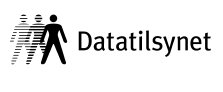
\includegraphics[width=0.7\linewidth]{./FurtherWork/img/Datatilsynet}
  \caption{Datatilsynet}
  \label{fig:FurtherDatatilsynetLogo}
\end{figure}

\subsection{Text Post}
\label{subsec:FurtherRequiredTextPost}
In the early stages of the project a feature enabling users to comment directly on a spot on the map was discussed. This feature will provide the opportunity to inform about places when no relevant picture is readily available. Since this will broaden the appeal of the system we believe it should be included. This feature will function in much the same way as the pictures and videos with users being able to rate and comment on the original text comment.

\subsection{Video}
\label{subsec:FurtherRequiredVideo}

A form of content that was not prioritized for the prototype but should be included in the system nevertheless is user created videos. Including this would not be a lot of work as much of the existing functionality for picture posts could be reused to enable the upload and displaying of videos. Like other forms of content users would be able to rate and comment on videos and they would be placed on the map and be searchable in the same way as pictures and events are handled in the current system. Video content will be more demanding on the server requirements both regarding bandwidth and space, than text or pictures are.

\subsection{Events}
\label{subsec:FurtherRequredEvents}

The event feature needs to be developed further. As mentioned in \ref{subsec:FurtherRequiredLacking}, the attend function must be completed to allow users to see events they are signed up for and to make events display how many people are participating. Further development of this feature could include a way to invite or notify a few users to minimize the chances of an event having only the organizer show up. If this form of feature is made as an invite then an option to respond with a “maybe” should be included. Depending on how the specific solution handles invitees who have yet to respond an option to decline the invitation might also need to be added.
\paragraph{} Additionally, the ability to view past events you have attended should be included. The ability to view these events can enable further discussion and increase exposure for that event in case a follow up is created, and it will make it possible for the organizers to learn from past experiences and improve their future events. This feature may also increase user enjoyment as it provides a way of centralizing content related to an arrangement, possibly stimulating memories of the event. This may also help users find other attendees they may have met on an event if they want to connect further with them.

\subsection{Moderation and Post-deployment Modification}
\label{subsec:FurtherRequiredMod}

Managing the system and ensuring that the content is appropriately relevant and inoffensive requires moderators to routinely check submissions and remove unwanted items. In order to make this task easier some privileges may be granted to users allowing them to report unwanted content for moderator review.  This will reduce the time necessary to identify content that should be removed. The moderators should also have be able to take punitive action against users who repeatedly violate the rules. This punishment may take the form of temporarily disabling some features of a user account, such as creating content or commenting. the specific options are something that should be worked out at a later stage when a more complete overview of the needs and problems of the site is available.

\paragraph{} To further empower users to deal with unwanted behaviour, all users should be able to edit or delete content they have created, and possibly remove specific comments made by other users on content they have created.

\paragraph{} As previously mentioned it is not feasible to include all relevant interests at launch, therefore users should be able to create interests they find are lacking. We believe that all new interests should be approved by a system moderator before they are included in the system to avoid superfluous or inappropriate tags. To this end, we suggest a feature where users can submit interests they think should be included to a central database. A list of all the pending interests should be viewable by users who can vote on the interests they think should be included, this should also count several submission of the same interest. When an interest is endorsed by a sufficient number of users it should be automatically sent to a moderator for approval. Interests that have already been refused should be permanently unavailable for such voting to avoid repeated rejection by the moderators.

\paragraph{} The reason we want voting rather than free creation of interests is that we do not believe a solution allowing users to freely create interests would be practical, both from a technical and a social point of view. The technical issues would include data fragmentation as a result of different spellings and names for the same interest, and different levels of specification. The social implications would be that an unmoderated solution  would ease the creation of unwanted interests like bullying, drug abuse, or other unwanted or criminal activity. As the project specifically tries to create safer social spaces this kind of solution may prove counterproductive.

\subsection{User Profile}
\label{subsec:FurtherRequiredUser}

Before launching the system, further development of the user profile is required. Currently the profile consists solely of username, password, gender, and full real name. Further information that could be stored in the user profile would include a user's favorite location and favorite interests. This information could be used to define the settings of the start page shown to the user upon logging on to the system. A customized search using the provided interests and area could be displayed when a user enters the system to increase the user's exposure to potentially interesting content. A feature to inform the user about arrangements related to their interests in their area in the near future could also be implemented, as part of a "suggested events" page, as this may make the system more appealing on a regular basis and help create user habits for checking the site every day.
\paragraph{} Additionally, a calendar feature displaying information about events a user has signed up for could be added as an easy way to get an overview of when different arrangements occur. This feature could also be expanded to alert users if they sign up to event scheduled at the same time.

\subsection{Mobile Application}
\label{subsec:FurtherRequiredMobile}

While the main focus of the project has been to develop a web platform, it was understood from the beginning of the project that a mobile application was needed if the product was to be a serious alternative to existing solutions. Based on the feedback reviewed in \ref{subsec:S2PresentationFeedback}, we decided to make a simple application to upload pictures to the system, but because of limited time the development of a full mobile application was not the top priority. However, before launch,  the project should offer a complete solution for at least the two most popular mobile platforms, Apple's iOS and Android. Because applications for these platforms are written in different programming languages it is necessary to make one for both, or find a framework, such as backbone.js, to develop for both platforms at the same time. If not using a framework, only the general design can be kept for both platforms, since the underlying design is different for each. Other, less popular platforms could also be considered in future.
\paragraph{} The feedback from potential end users in the T{\o}yen area in Oslo revealed that a significant portion of these users might not have access to a personal computer to access the functionalities of the web application. Therefore it is imperative that further development takes this aspect into consideration and delivers mobile applications that can function on their own without requiring users to interact with the web page, or develops the web page to work well on mobile platforms, possibly including an in-app browser as part of the early versions of the app.

\begin{figure}[ht!]
  \centering
  
\includegraphics[width=0.7\linewidth]{./FurtherWork/img/iOSAndroid}
  \caption{iOS and Android are the largest operating systems for mobile devices.}
  \label{fig:FurtherIOSAndroidLogo}
\end{figure}

\subsection{Security}
\label{subsec:FurtherRequiredSecurity}

The current product does not include any extensive security measures. Before the system can be launched measures must be implemented to ensure that user information is kept confidential and can not be easily retrieved and exploited. Encryption of user information is one of the necessary steps to take, to stop the data from being usable even if someone were to get their hands on it, providing an additional level of security against malicious attacks on the system.
\paragraph{} Another use for security measures would be to limit the vulnerability to automated user creation which could both serve to create unreasonably high workloads for the system and also to manipulate content and user statistics by creating many fake users. An easy preventive measure for this concern is to include the use of a CAPTCHA (Completely Automated Public Turing test to tell Computers and Humans Apart) in the account creation process. A CAPTCHA will reduce the feasibility of automatically creating users by utilizing a script, and thus help ensure that no large-scale sabotage can occur as a result of large amounts of fake users.
\paragraph{} Security procedures could also be used to provide account services such as password retrieval. To this end it would be advantageous to expand the current account version to also include a user email, this may be implemented as either a required feature or as an optional one. In any case the linked email can be utilized to recover account information as well as a possible venue for receiving information about potentially interesting activity for users.

\subsection{Scaling}
\label{subsec:FurtherRequiredScaling}

It is important that the system can support a large amount of users simultaneously. To this end some of the solutions in place at the moment may have to be changed to better facilitate system scalability. The system might require additional servers and it is imperative that adding these is a smooth and easy process. This again requires that all the code is written with scalability of the system in mind. The need for more servers might present itself as a consequence of the quantity of content increasing, as the number of pictures, but especially videos on the site goes up more server space might be required.
\paragraph{} The current system features a very limited amount of interests. Adding more before deployment is needed but even so it is probable that not all interests will be covered. Therefore the previously mentioned adding of popular suggested interests will be important to deliver a service that corresponds to the needs of the users. Adding additional interests should be easy and, while we believe the suggested interest should be manually approved, the method of submitting and adding new interests could be highly automated.
\paragraph{} A different consideration when it comes to this is the use of the Google Maps API. According to the licence agreement Google reserves the right to demand payment if the site “generates more than 25 000 map loads or more each day for more than 90 consecutive days”. The map loads relevant for this project occurs when a map is displayed using the Maps JavaScript API and when a single request is made for a map image from the Static Maps API. As these limits might be reached on a daily basis with a few thousand users the system should monitor how many are generated each day, and consider the options available for solving this problem. One way to do it might be to create a unique map solution for the system, however this would be very costly to develop and we do not recommend this way of solving the problem.
\paragraph{} For sites exceeding the limit Google offers two different payment solutions. One is to pay 0.50 USD for every 1000 excess map loads, while the other is to purchase a Google Maps API for Work. The Google Maps API for Work option also delivers many other services besides unlimited map loads. The use of user growth projections as well as statistics regarding how many map loads are generated per user each day on average should be used when deciding which option to use. While this may become a consideration even with a small amount of users, it is impractical to give further advice on the matter without statistics from a system in use with a considerable amount of users over a substantial time frame. \cite{website:maps-api-docs-usage,website:maps-api-faq}

\begin{figure}[ht!]
  \centering
  
\includegraphics[width=0.9\linewidth]{./FurtherWork/img/GoogleDevelopersLogo}
  \caption{Google provides the API for the map used in the product.}
  \label{fig:FurtherGoogleDevelopersLogo}
\end{figure}

\subsection{Implementation Time Estimates}
\label{subsec:FurtherRequiredEstimate}

In order to create a system with the features discussed above in addition to the ones existing currently a lot of work is required. The time needed to complete the product would depend on several factors. 
\paragraph{} First, the competence and experience of the development team influences the overall productivity of the project which then again influences the time needed for completion. Second, the team motivation also influences productivity. Third the stability of the system requirements affects the time needed as drastic changes in the requirements may lead to some work being rendered useless for the final product. Additionally some features of the product require expertise beyond that readily available to a normal computer engineer such as knowledge of legislation and design. When some tasks are dependant on external work in this fashion, unforeseen delays may result if the expert is otherwise occupied or delayed in some way. Finally both the specific solutions to some problems the degree of inclusion of additional features may result in a workload variance. 
\paragraph{} These factors combined makes it difficult to give a precise estimate for completing the product. For ease of estimation two estimates will be provided, one based on our group and one with a hypothetical perfect team. For developing a complete system for web browsers, iOS, and Android with adequate modifiability and security measures to service a large user base and keep the system stable and reliable, based on the current product our group would require approximately 2700 additional work hours. For an ideal team consisting solely of the most experienced expert developers working under ideal conditions creating the entire system from scratch would require approximately 2400 work hours. All estimates are made using the use case based tool provided in the course compendium, Appendix F. \cite{booklet:CDPCompendium}.
\paragraph{} It is important to note that the product made in this project is a prototype and that some of the underlying features might have to be redone to meet the quality standards of a large social network. This means that while the product can be a useful illustration of parts of a complete system, it may not be ideal as a core system for further development.

\section{Possible Improvements}
\label{sec:FurtherImprovements}

This section details features we believe to be advantageous to the system and should be included eventually but that are not necessarily required for a launch.

\subsection{Improve Visual Design}
\label{subsec:FurtherImprovementsVisDesign}

The visual design of the page is something we believe can be improved in the future. As no member of the group is a professional designer and the usability testing was limited during the project, the design was not the main feature in focus. When further developing the visual appearance of the site, more advanced solutions involving interactive features can be included to further increase the visual appeal to target users. Such features could include animated menus and buttons providing instant visual feedback for users. We recommend seeking professional consultation on visual elements in the future to deliver the best possible user experience.
\paragraph{} Merging the different kinds of posts into one feed may be considered, at least in some places. However as the quantity of posts increase this may provide little benefit as the feed may be filled up with a lot of unwanted content. This would also require a slight reworking of rankings, to make all posts follow the same system.

\subsection{Enabling User Interaction}
\label{subsec:FurtherImprovementsInteraction}

End user feedback, found in \ref{subsec:S2PresentationFeedback}, indicates a desire to view and interact with other users on a more personal level. Several measures may be taken to facilitate such user interaction. The most obvious way is to implement some form of user to user private communication. The exact form of this messaging service could be either direct chat or a private message. More user feedback should be collected to find out which of these solutions is more desirable.
\paragraph{} Another feature that could improve on this aspect is the creation of a public user profile page. The current focus is on the content and active use of the system in order to meet new people, and not on providing extensive support for communication beyond that, as we believe other services, such as Facebook or the exchange of phone numbers, will be preferable in any event. However, as the system matures user profile pages might be a desired addition. This could open new possibilities by allowing users to see, and maybe also subscribe to, events and other content created or interacted with by other users.
\paragraph{} A feature that could help create communities in the system would be to include pages for interests where media and discussions related to the interest could be found. These pages should include the most popular posts related to the interest in question regardless of the types of content. This may also be a smart place to include live streams if or when that feature is included in the system. This feature provides a centralized hub for an interest and may help generate interesting discussions and connect people with similar interests regardless of other differences such as physical distance. %TODO More examples?

\subsection{Customized Presentation of Content}
\label{subsec:FurtherImprovementsCustomized}

A feature that should be included to enhance the browsing experience would be different ways to sort the content beyond filtering by interests and location. The current sorting for pictures is based on how old any particular piece of content is while still taking into consideration how popular it is (see equation~\ref{eq:S5DesignImplSorting} on pave~\pageref{eq:S5DesignImplSorting}). However, time is several orders of magnitude more important when generating the overall rating of posts. This may not be optimal as different content may be relevant for users for disparate time intervals; a football field would be relevant for as long as it exists, while the location for a concert would not be relevant after the concert was over.
\paragraph{} In order to improve the user experience several different modes of sorting might be considered. One option would be to enable sorting by popularity, this option might have a time window as an additional parameter allowing users to view the most popular content from the last week, month or since the service started. This mode could be complemented with a mode of viewing content based only on creation date with newest content being listed first. Additionally further tweaking of the current solution might be considered, adjusting the relative importance of popularity in comparison to the time since a post was created.
\paragraph{} Sorting criteria could also be dependent on the type of content in question, for events the time of the event could be factored in as well as the percentage of participation registered on the site. In addition a feature enabling users to find events with at least a certain numbers of free slots should be considered. Videos could have an option allowing them to be sorted on length in addition to the other criteria.
\paragraph{} It would also be possible to analyze the user activity of a registered user and create a recommendation system which could predict what types of  content that user might enjoy and present the most popular matching results, this could also take into consideration the location and interests of a user. This feature might also be implemented separate from the normal feed view. The information used to calibrate this would need to be mentioned in the legal document for user review. As users must agree to the tracking and saving of relevant information to enable accurate results the recommendation section would only be available to registered users. Agreeing to use this function should not be mandatory to create a functional user account.

\subsection{The Digital Stage} 
\label{subsec:FurtherImprovementsStage}
One of the ideas the customer presented was to create a digital stage with live streaming of any performances held there. A feature like this could help create a sense of community and make users feel more connected to each other despite physical distances. It would also provide a channel for young musicians and other performers to generate exposure and interest for their work and possibly help them further their careers. We feel that this feature would be a good way to differentiate the product from other social media and recommend that it is implemented in the future. When communicating with potential users this idea was also highlighted as one of the most interesting features and one of the big incentives to use this service in the future. 
\paragraph{} In order to provide a real time broadcast a streaming server is required. Operating a streaming server can be very costly and therefore contacting existing services and purchasing a hosting plan for streaming, is probably a superior alternative and should be considered, at least in the early phase. Another possibility is to use an already existing solution to do the streaming, rather than just purchasing hosting, and embed that stream in the page. The page \href{feat.fm}{http://www.feat.fm}, made for streaming concerts live on the site, was made by NTNU students by embedding a stream solution made by \href{ustream.tv}{http://www.ustream.tv}, and such a solution seems very usable in this case as well.
\paragraph{} Another thing to consider is the availability of this stream. Either the people on stage, or the stage owners might wish to limit availability based on certain criteria, such as location. Users who do not fulfill those criteria may not get to view the content, or the content may be of lower quality. Note that there is no foolproof way of finding someone's location. The system simply has to trust that the ip address it is given is correct, and a proxy could easily fool it. However, this is beyond the skill set of most users, and should only be a very minor problem.